\section{Comparison of NLP Transformer Models}
\label{sxn:nlp}

\paragraph{GPT vs GPT2}

\begin{table}[t]
\small
\begin{center}
\begin{tabular}{|p{1in}|c|c|c|c|c|}
\hline
   &    & Frobenius Norm & Spectral Norm & Weighted Alpha & Alpha-Norm \\
 Series & \#Layers   & $\Vert\mathbf{W}\Vert_{F}$ & $\Vert\mathbf{W}\Vert_{\infty}$ & $\hat{\alpha}=\alpha\log\lambda_{max}$ & $\Vert\mathbf{X}\Vert^{\alpha}_{\alpha}$ \\
\hline
 GPT & & & & \\
 GPT2 (small) & & & & \\
 GPT2-medium & & & & \\
 GPT2-large & & & & \\
 GPT2-xls & & & & \\

\hline
\end{tabular}
\end{center}
\caption{Average metrics for pretrainnd OpenAI GPT and GPT2 models.}
\label{table:models}
\end{table}


\paragraph{Power Law Exponents}

\begin{figure}
   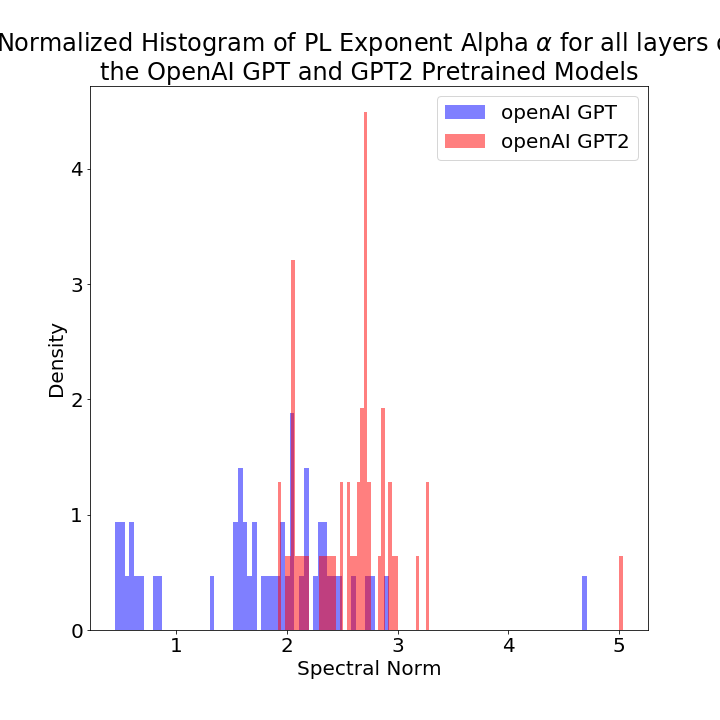
\includegraphics[scale=0.25]{img/gpt-alpha-hist.png}
   \caption{Comparison of heavy tailed power law exponent $\alpha$ for OpenAI GPT and GPT pretrained models}

   \label{fig:gpt-alphs-hist}
\end{figure}


\begin{figure}[t]
    \centering

    \subfigure[ Power Law Exponent $\alpha$  ]{
        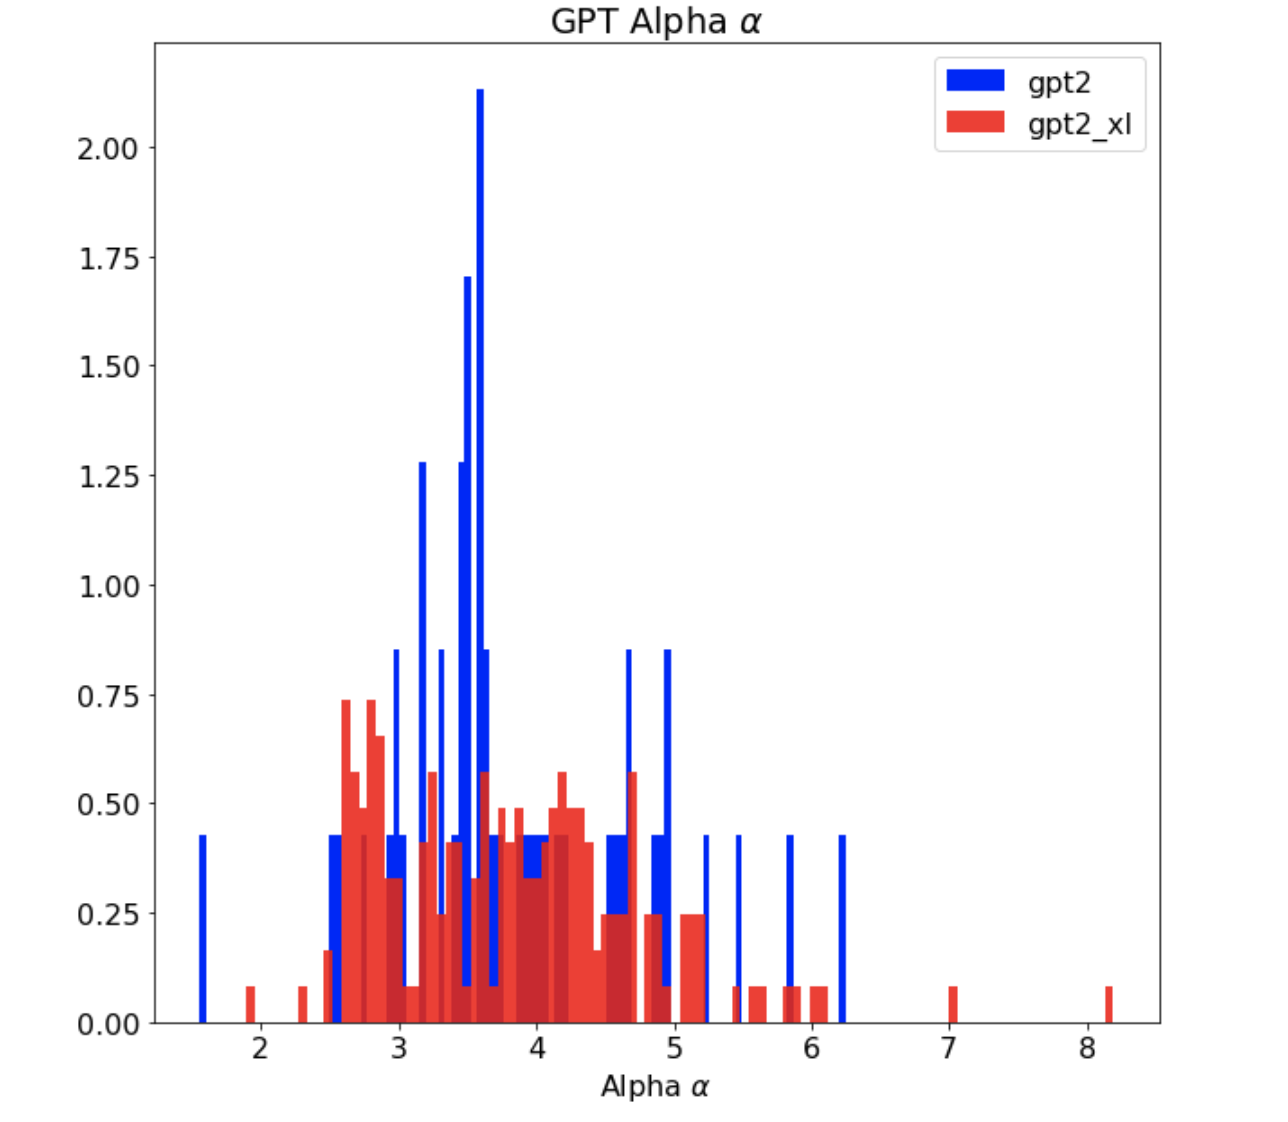
\includegraphics[width=4.5cm]{img/gpt2-alpha-hist.png}
        \label{fig:gpt-alpha-layer}
    }
    \qquad
    \subfigure[ Spectral Norm $\Vert\mathbf{W}\Vert_{\infty}$]{
        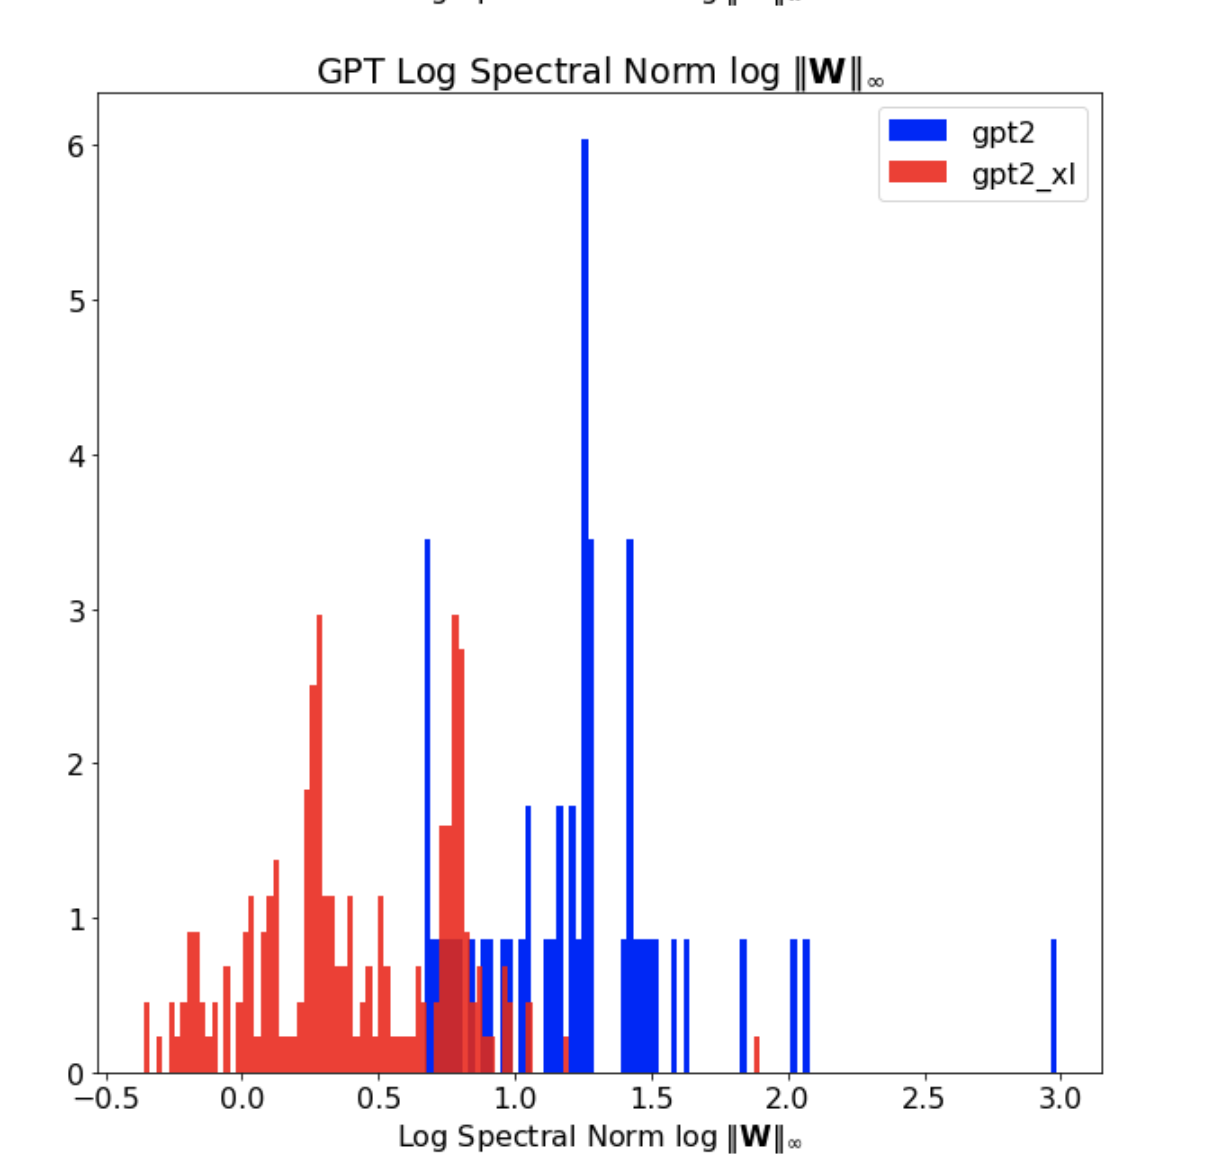
\includegraphics[width=4.5cm]{img/gpt2-snorm-hist.png}
        \label{fig:resnet-snorm-layer}
    }
    \qquad
    \subfigure[ Alpha-Norm $\Vert\mathbf{X}\Vert_{\alpha}^{\alpha}$]{
        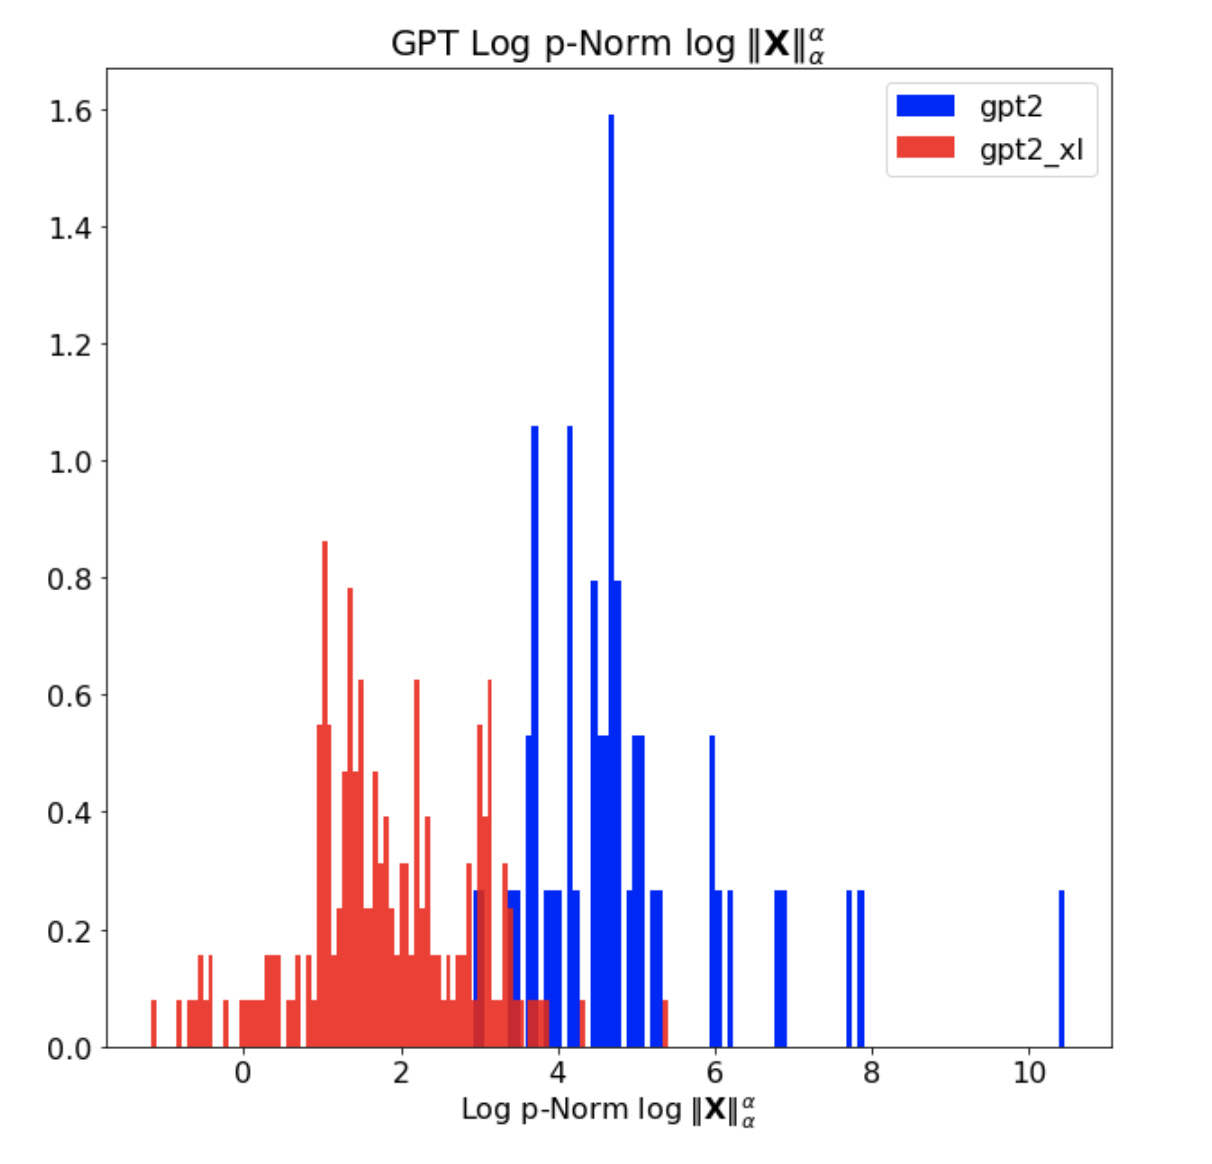
\includegraphics[width=4.5cm]{img/gpt2-pnorm-hist.png}
        \label{fig:gpt-pnorm-layer}
    }
    \caption{Comparison of Power Law Exponnents, Spectral Norm, and Alpha-Norm for different size models in the GPT2 architecture series.    }
    \label{fig:gpt-alpha-layers}
\end{figure}


\paragraph{Correlation Flow}

\begin{figure}[t]
    \centering

    \subfigure[ Power Law Exponent $\alpha$  ]{
        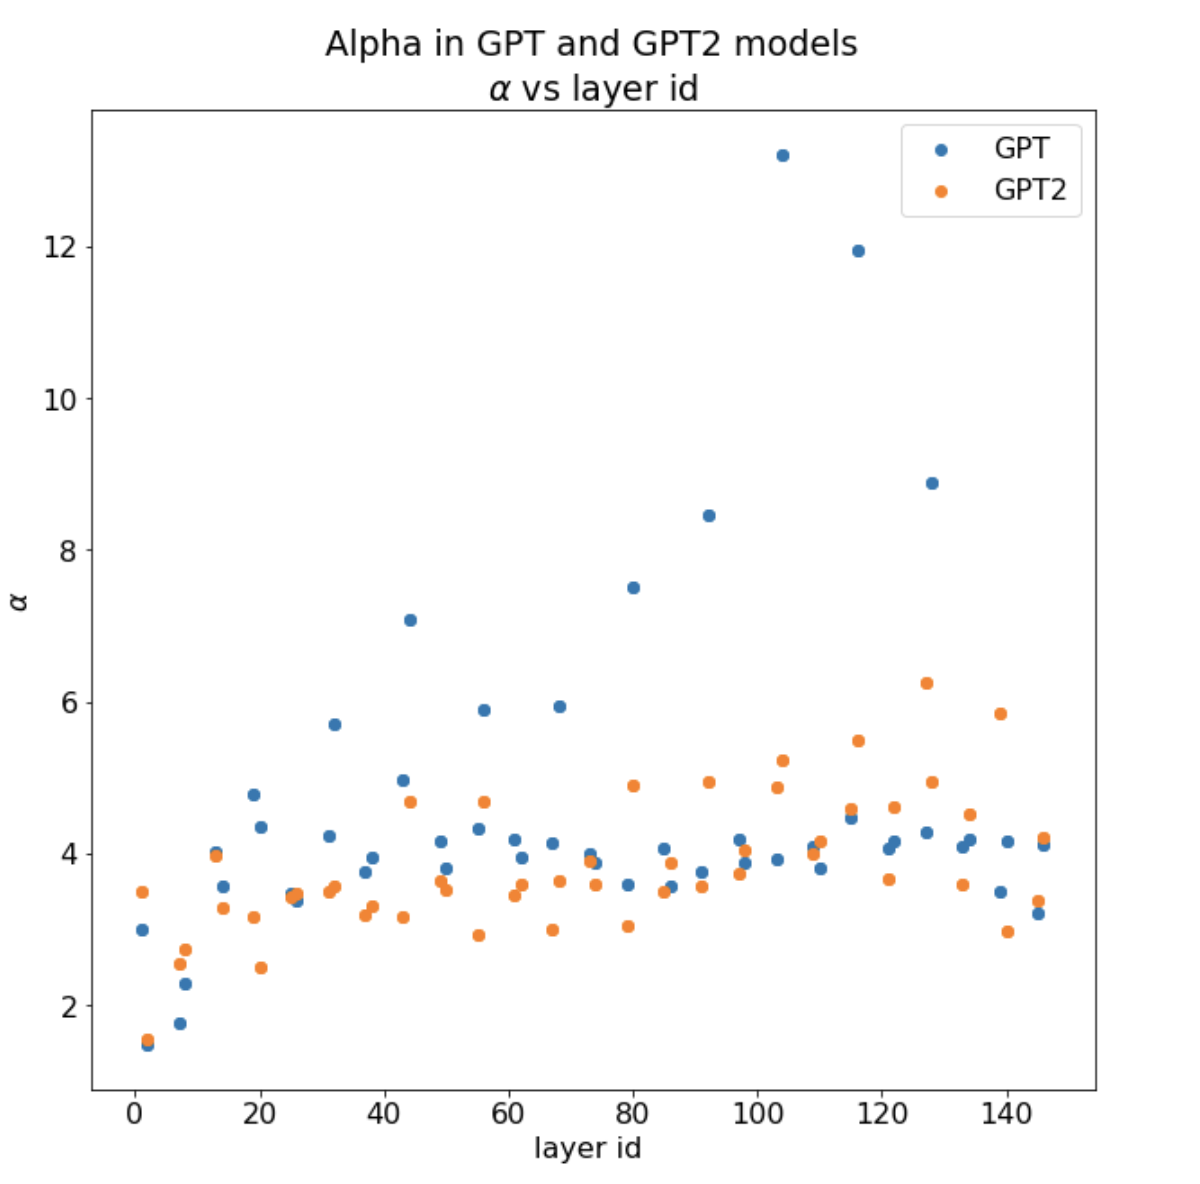
\includegraphics[width=4.0cm]{img/gpt-alpha-layer.png}
        \label{fig:gpt-alpha-layer}
    }
    \qquad
    \subfigure[ Spectral Norm $\Vert\mathbf{W}\Vert_{\infty}$]{
        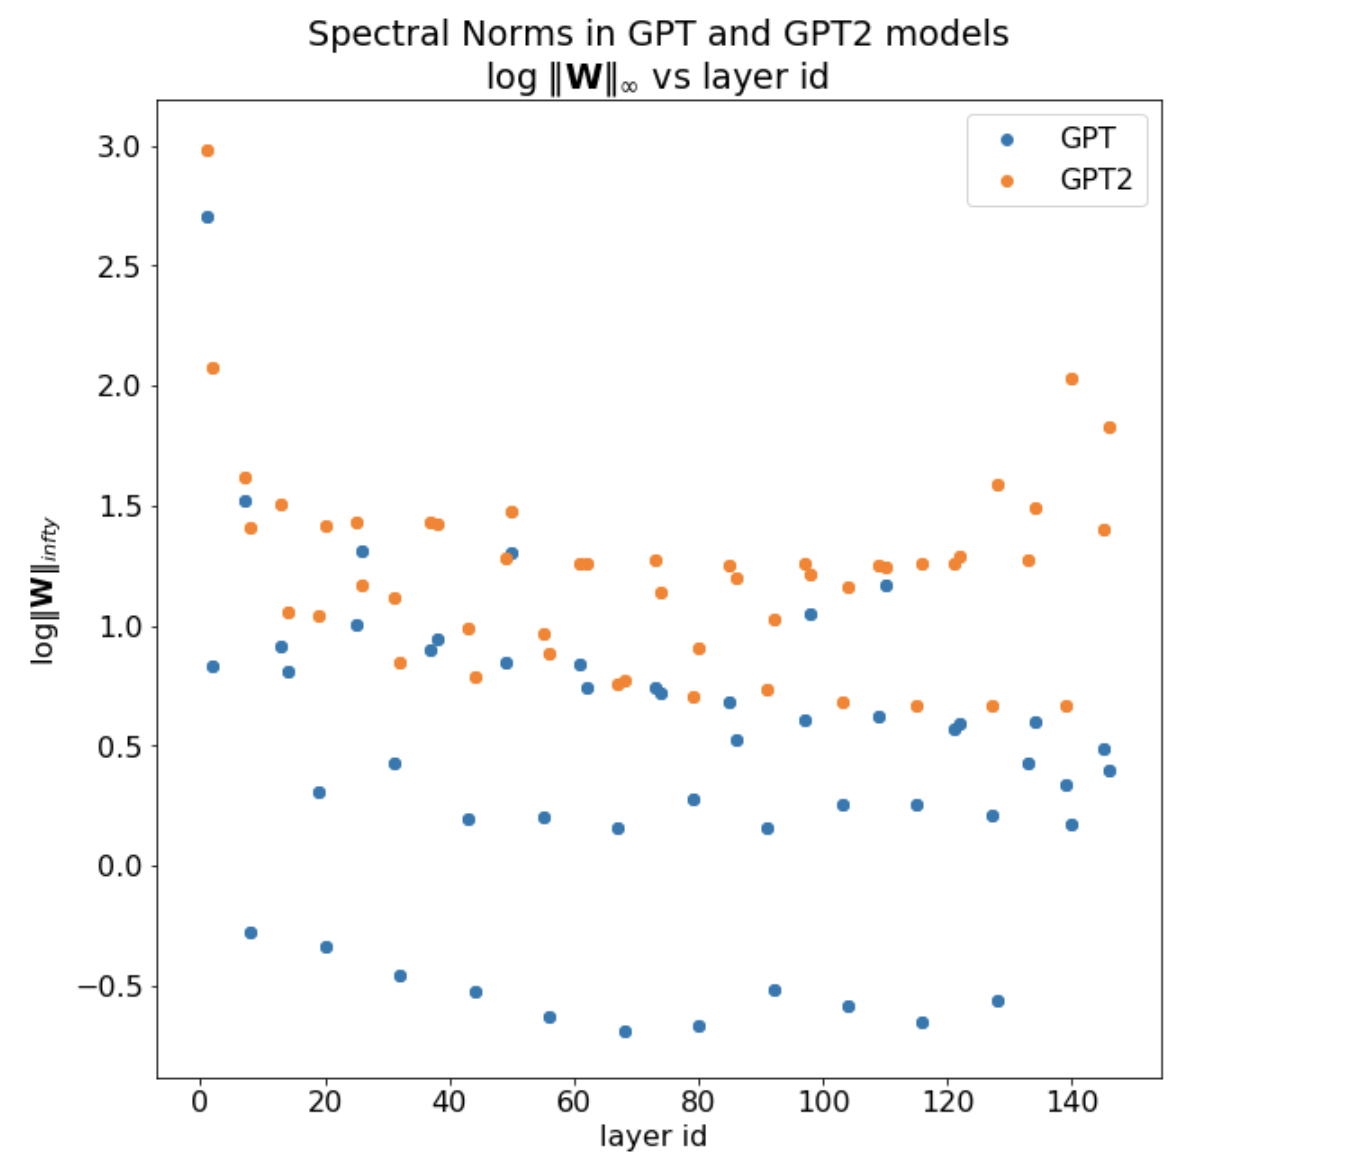
\includegraphics[width=4.5cm]{img/gpt-snorm-layer.png}
        \label{fig:resnet-snorm-layer}
    }
    \qquad
    \subfigure[ Alpha-Norm $\Vert\mathbf{X}\Vert_{\alpha}^{\alpha}$]{
        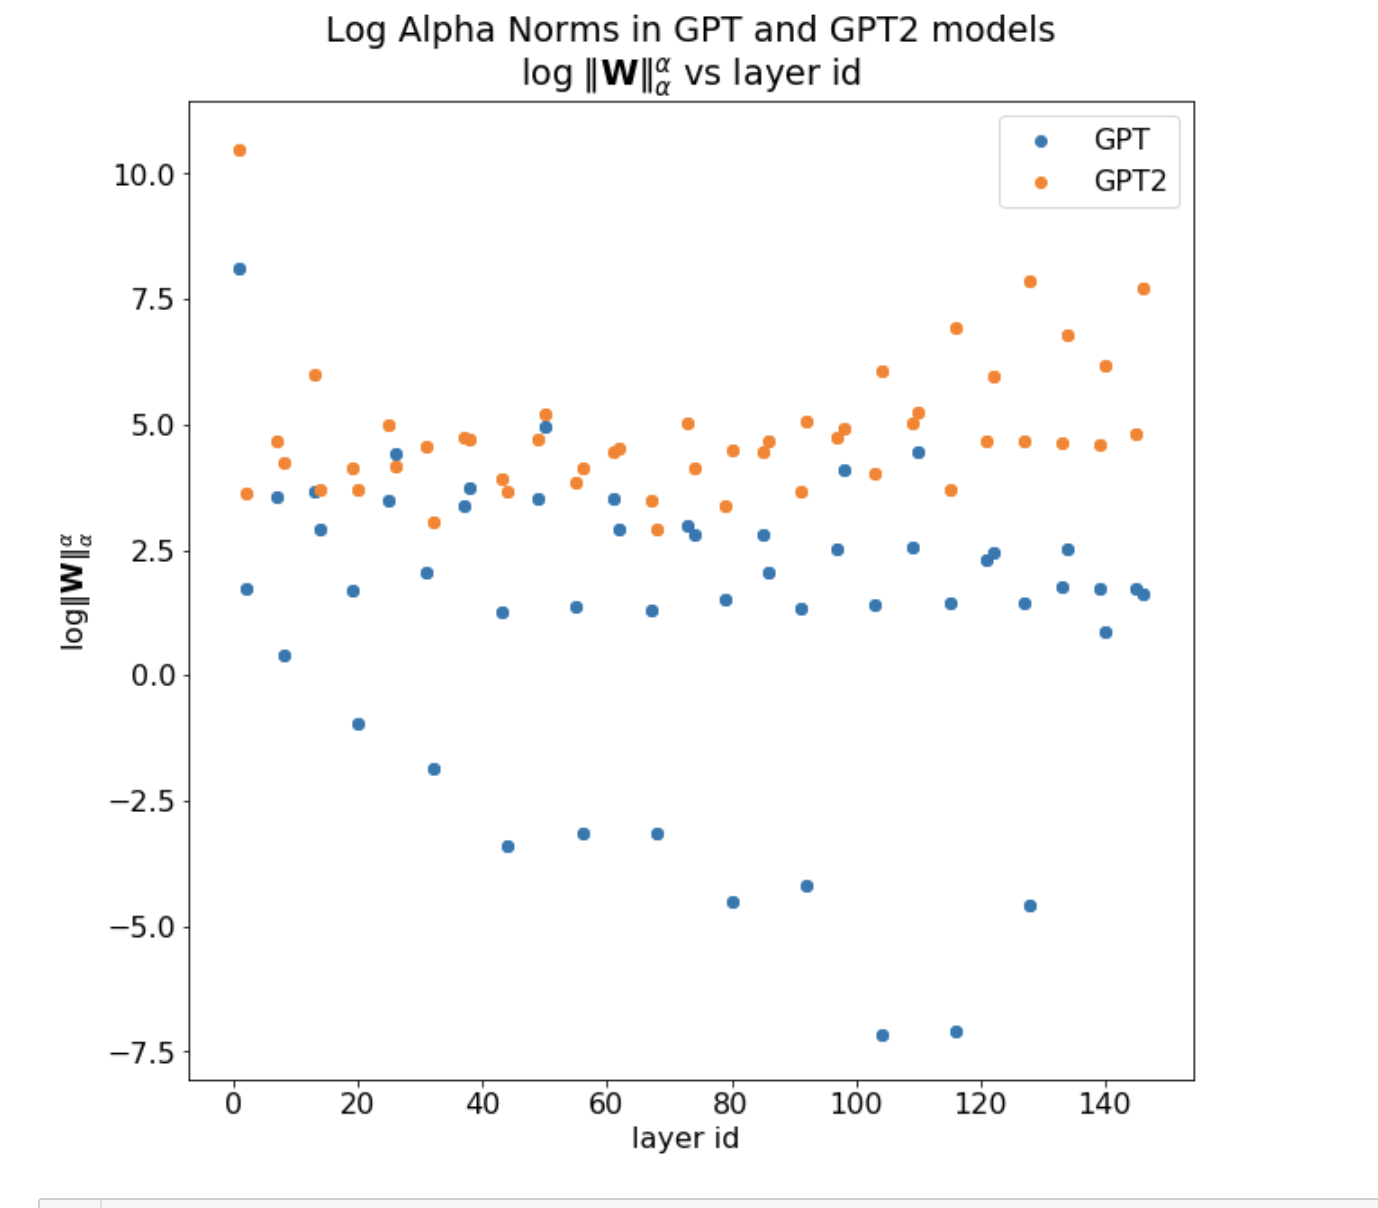
\includegraphics[width=4.5cm]{img/gpt-pnorm-layer.png}
        \label{fig:gpt-pnorm-layer}
    }
    \caption{Comparison of Correlation Flow and Spectral Norm for OpenAI GPT and GPT2   }
    \label{fig:gpt-alpha-layers}
\end{figure}

\paragraph{GPT2: small, medium, large, extra-large}



